\section{Background Studies}
 \label{sec:background}
In order to distinguish the Higgs boson signal from the background using \dm
as a discriminant, a model for the background distribution is needed. The background
is modeled with a smooth analytic p.d.f. that reproduces the data as well as the 
mixture of background Monte Carlo samples normalized to the data-driven background 
yields. It should be noted that the parameters of the background p.d.f. are not fixed
from simulation, but are fitted on the data. The model was chosen carefully so that
it does not introduce significant biases on the fitted signal while at the same
time preserving the sensitivity to the search.

\subsection{Background Model}
A number of functional forms were tested including polynomials of various orders,
as well as non-polynomial functions such as exponential, Crystal Ball+Gaussian,
and Crystal Ball+Landau distributions. The advantage of non-polynomial functions
is that they do not follow the local peaks and troughs of the mass distribution 
that are a result of statistical fluctuations. A high statistics simulated
background-only Monte Carlo sample was used to test the performance of the
signal+background fits of the \dm distribution. This was done by performing
pseudo-experiments\footnote{Data generated by sampling from a known distribution
using a Monte Carlo sampling method. 
The resulting distribution looks like data from the experiment.} 
with a variable amount of Higgs signal events injected in
the mass range 115-135 GeV. For each experiment an unbinned maximum likelihood
fit is performed for a fixed \mllg, and the number of signal events together
with the fitted parameters are obtained. The key result of these tests is
the \emph{spurious signal}, i.e. the bias on the signal. The spurious signal
is defined as the average fitted number of signal events after subtracting
the input signal events ($\average{S} - S_{\text{generated}}$) in units of the
uncertainty in the fitted number of signal events, $\sigma_S$. In order for the
spurious signal to not give a systematic uncertainty on the final result
that is significant compared to the statistical uncertainty of the measurement
itself, we searched for models that yield, for the tested Higgs mass hypotheses,
a spurious signal which is within $\pm20\%$ of the fitted error on the signal yield.

The results for the background-only simulated samples corresponding to $4.6 \ifb$
of 2011 data and $21 \ifb$ of 2012 data in the muon and electron channels are
shown in \refF{fig:spurioussignal}.The model that was found to provide the best 
sensitivity to the signal while limiting
the spurious signal to be within $\pm20\%$ of the fitted signal uncertainty, for
both $4.6 \ifb$ of 2011 data and $20.7 \ifb$ of 2012, is a third-order 
Chebychev polynomial in the fit range $24 < \dm < 64 \GeV$.

\begin{figure}[htbp]
    \centering
    \begin{subfigure}[b]{0.45\textwidth}
      \centering
      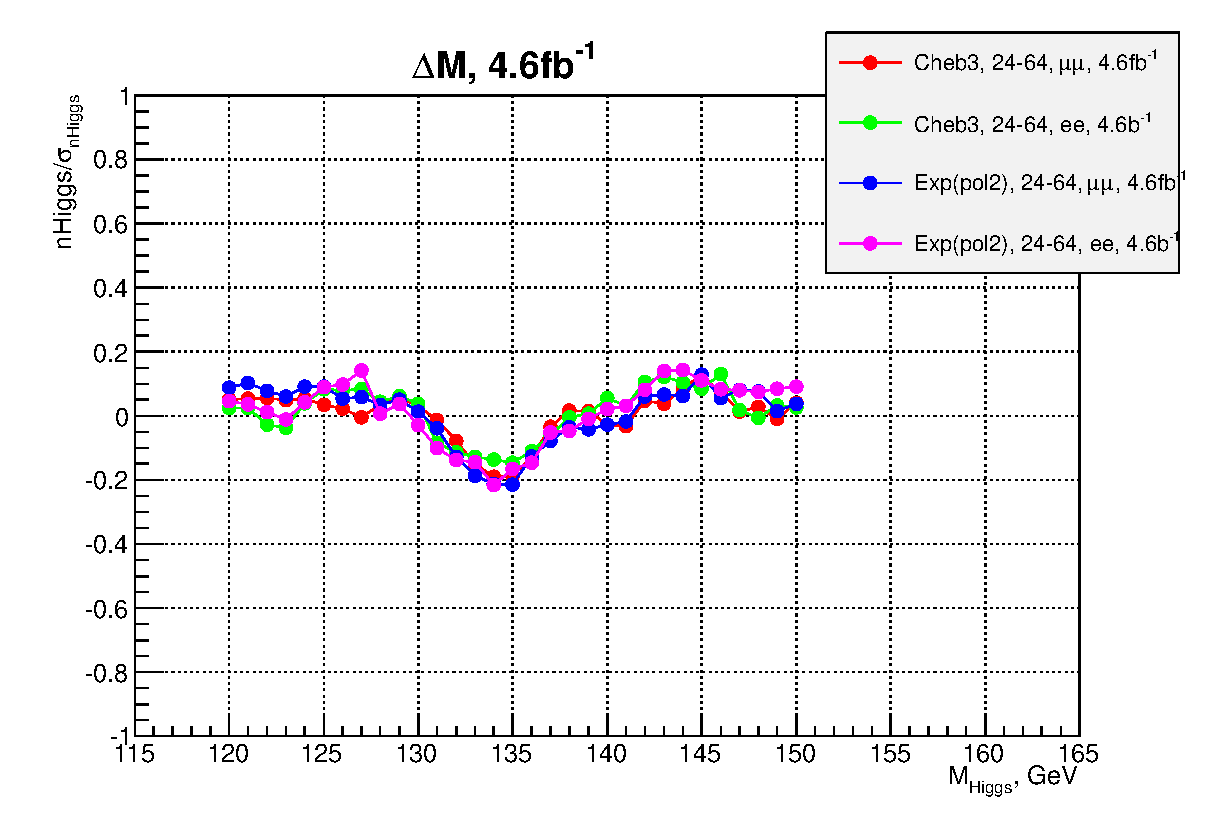
\includegraphics[width=\textwidth]{figures/rat4orig.eps}
      \caption{}
      \label{fig:4spurious}
    \end{subfigure}
    \quad
    \begin{subfigure}[b]{0.45\textwidth}
      \centering
      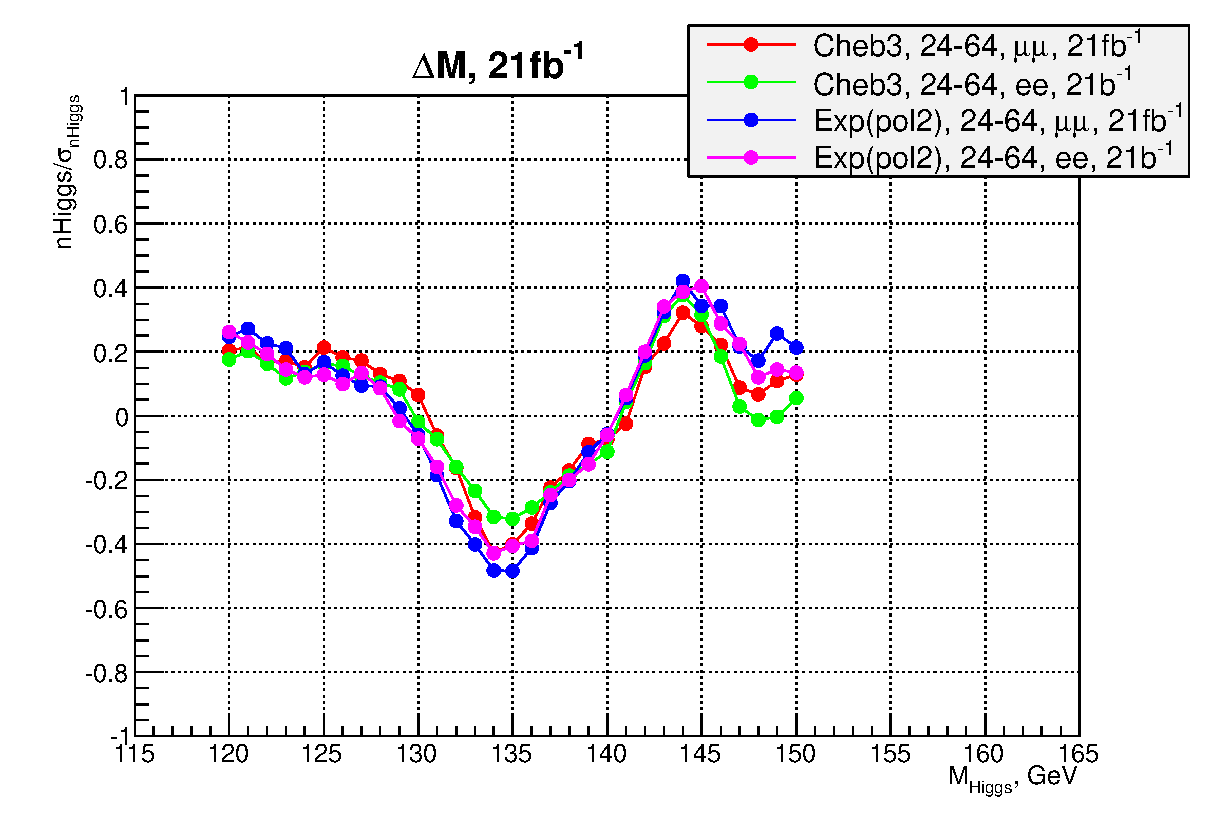
\includegraphics[width=\textwidth]{figures/rat21orig.eps}
      \caption{}
      \label{fig:21spurious}
    \end{subfigure}
    \caption{Number of Higgs candidates divided by uncertainty 
    returned by the fit of the pseudo-data $\Delta M$ distributions averaged over 
    1000 pseudo-experiments with 0 injected Higgs candidates. 
    The statistics corresponds to 4.6 \ifb (Fig.~\ref{fig:4spurious})
    and 21 \ifb (Fig.~\ref{fig:21spurious}). The dip at 135 GeV in the
    $21 \ifb$ sample is due to downward fluctuation in the data at this mass.}
    \label{fig:spurioussignal}
\end{figure}

\subsection{Background-Only Fits to the Data}
The shape parameters and the normalization of the background are determined
by unbinned maximum likelihood fits to the data events selected in the
range $24 \GeV < \dm < 64 \GeV$, performed separately for the two lepton categories
and separately for the $\rts = 7 \TeV$ and $\rts = 8 \TeV$ data, using the third-order
Chebychev polynomial selected in the previous section. 
\refF{fig:deltaM_data_bkgonly_fit} shows the background-only fits to the data in the
two categories for the $\rts = 7 \TeV$ and the $\rts = 8 \TeV$ data.

 \begin{figure}[!htbp]
  \begin{center}
    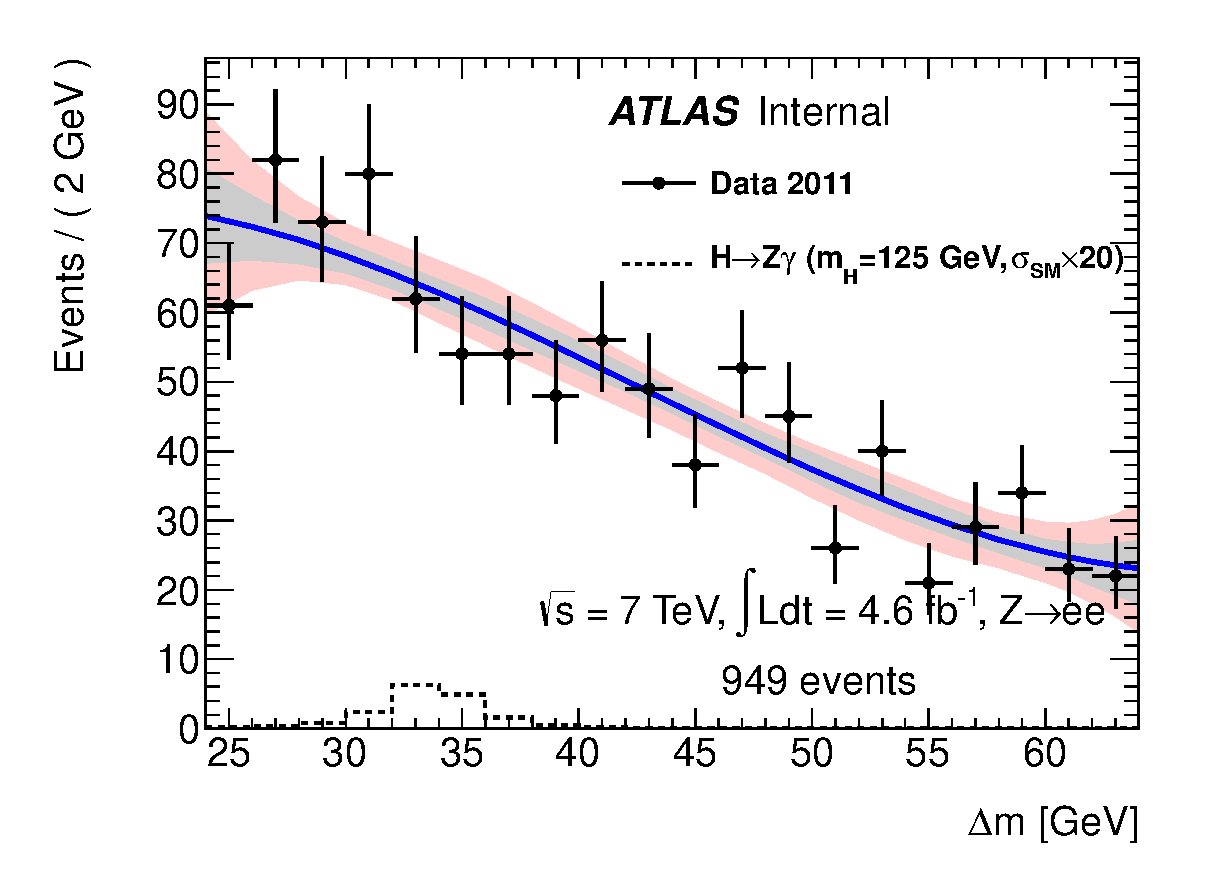
\includegraphics[width=0.49\columnwidth]{figures/bkgplots_e_deltaM_fit_11_CB3_fiterr_internal_withsignal}
    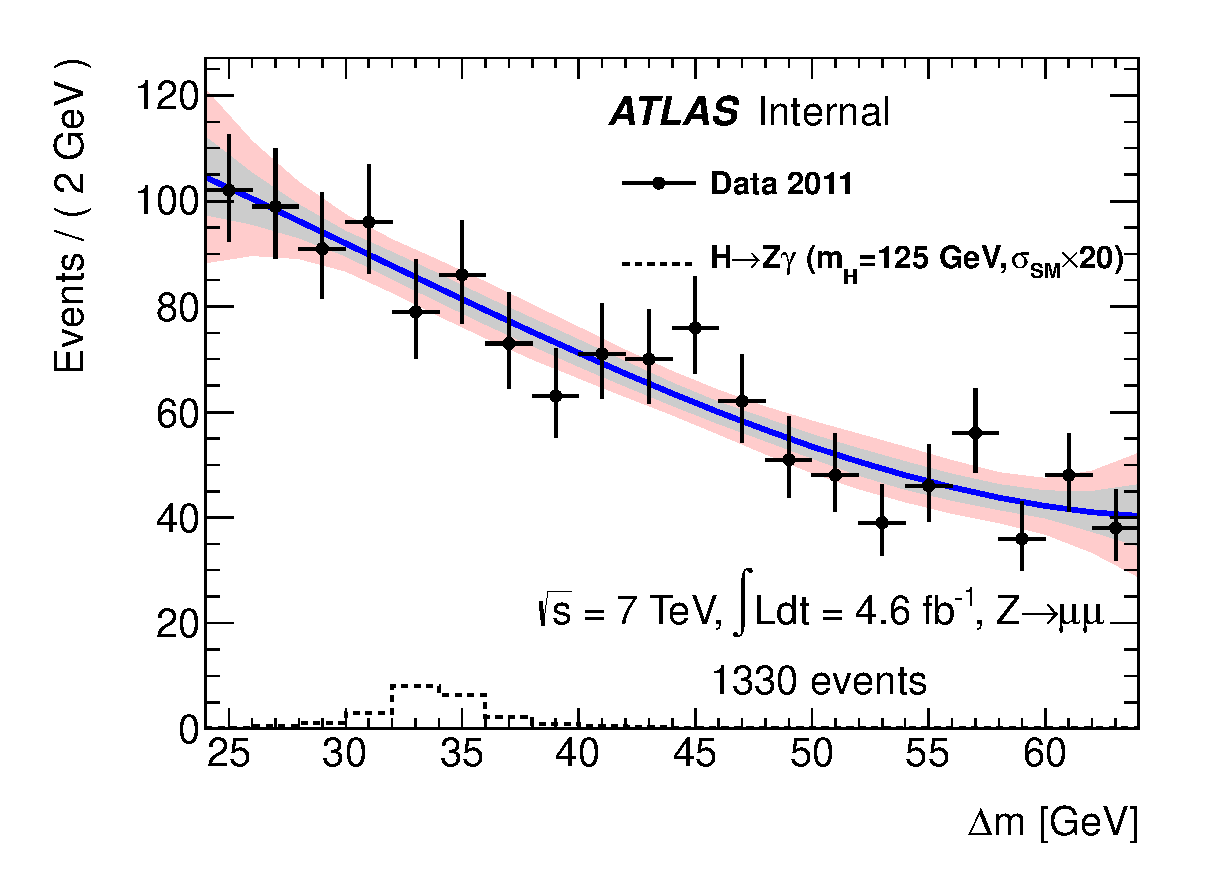
\includegraphics[width=0.49\columnwidth]{figures/bkgplots_mu_deltaM_fit_11_CB3_fiterr_internal_withsignal}
    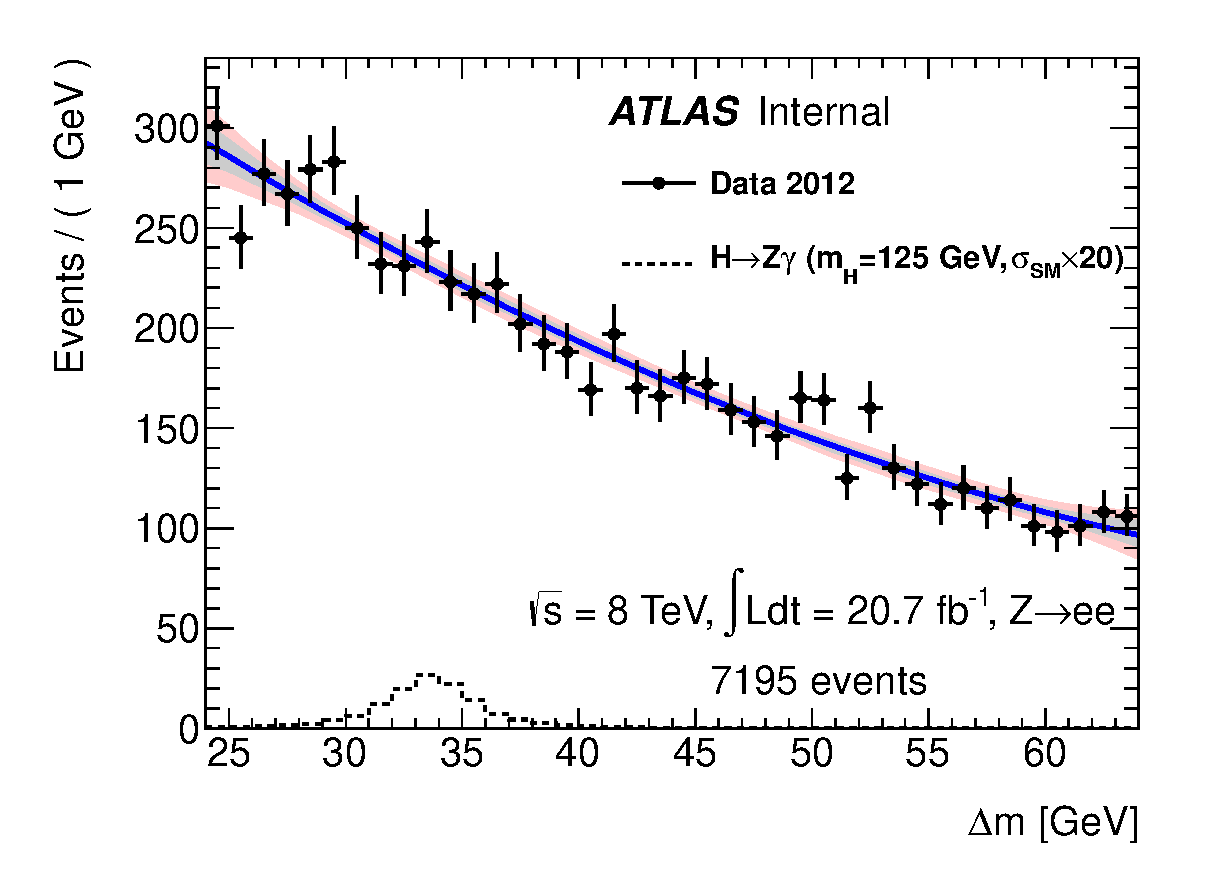
\includegraphics[width=0.49\columnwidth]{figures/bkgplots_e_deltaM_fit_12_CB3_fiterr_internal_withsignal} 
    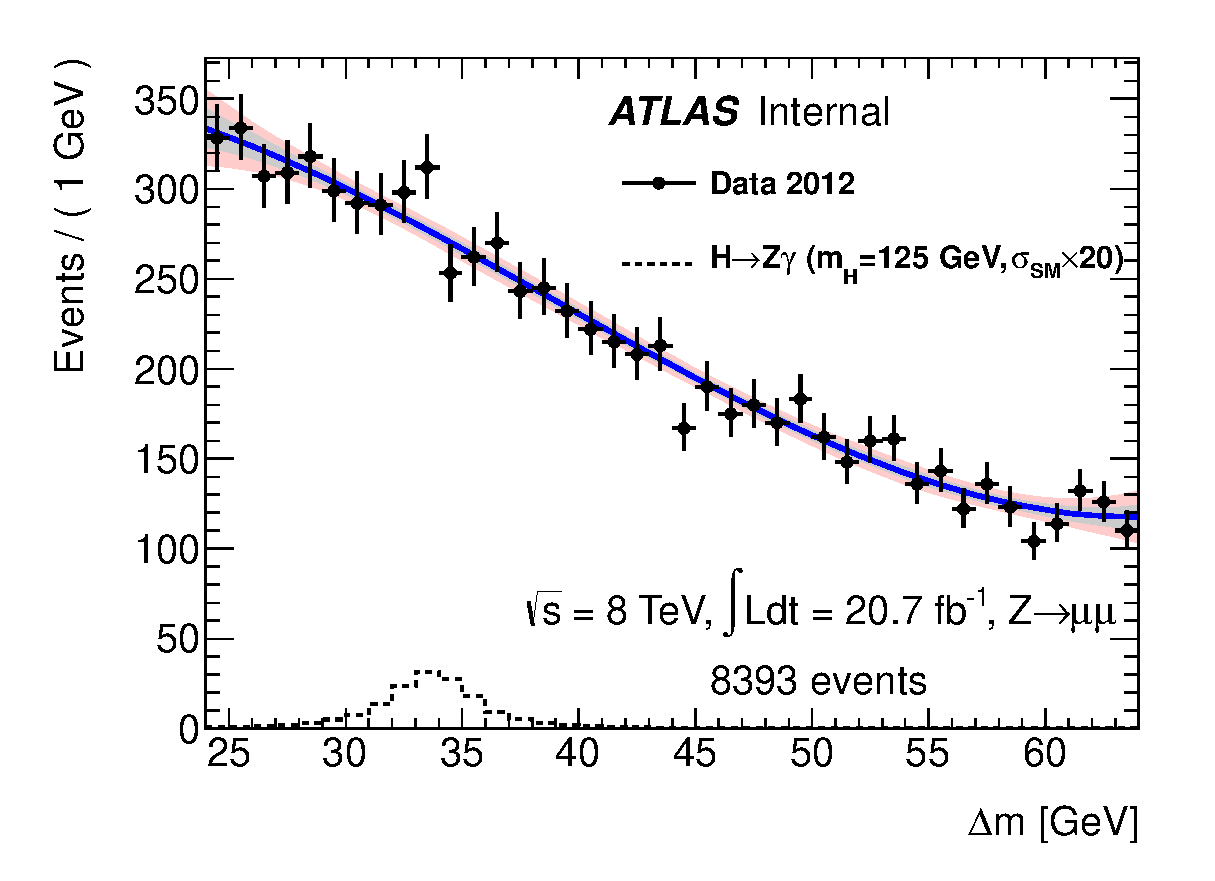
\includegraphics[width=0.49\columnwidth]{figures/bkgplots_mu_deltaM_fit_12_CB3_fiterr_internal_withsignal}
    \caption{Background-only fits to the distribution of 
      the mass difference $\Delta m$ of selected events in data,
      for $Z\to ee$ (left) and $Z\to\mu\mu$ (right), at $\sqrt{s}=7$ 
      TeV (top) or 8 TeV (bottom).
      For both 7 and 8 TeV, a third order polynomial is used for the fit.
      Dots correspond to data, the blue line is the fit result and the gray and light red
      bands are the 1$\sigma$ and 2$\sigma$ uncertainty 
      bands from the statistical uncertainties on the fitted 
      background model parameters.
      The dashed histograms correspond to the SM signal expectation,
      for a Higgs boson mass of 125 GeV, scaled by a factor 20 for clarity.
%%      The pulls of the data points with respect to the fit are also shown.
    }
    \label{fig:deltaM_data_bkgonly_fit}
  \end{center}
\end{figure}
